	\documentclass[12pt]{article}
\usepackage{color}
\usepackage{mathtools}

% This first part of the file is called the PREAMBLE. It includes
% customizations and command definitions. The preamble is everything
% between \documentclass and \begin{document}.
\usepackage{amsmath}
\usepackage[margin=1in]{geometry}  % set the margins to 1in on all sides
\usepackage{graphicx}              % to include figures
\usepackage{amsmath}               % great math stuff
\usepackage{amsfonts}              % for blackboard bold, etc
\usepackage{amsthm}                % better theorem environments
\usepackage{changepage}
\usepackage{lipsum}                     % Dummytext
\usepackage{xargs}                      % Use more than one optional parameter in a new commands
\usepackage[pdftex,dvipsnames]{xcolor}  % Coloured text etc.
% 
\usepackage[colorinlistoftodos,prependcaption,textsize=tiny]{todonotes}
\newcommandx{\unsure}[2][1=]{\todo[linecolor=red,backgroundcolor=red!25,bordercolor=red,#1]{#2}}
\newcommandx{\change}[2][1=]{\todo[linecolor=blue,backgroundcolor=blue!25,bordercolor=blue,#1]{#2}}
\newcommandx{\info}[2][1=]{\todo[linecolor=OliveGreen,backgroundcolor=OliveGreen!25,bordercolor=OliveGreen,#1]{#2}}
\newcommandx{\improvement}[2][1=]{\todo[linecolor=Plum,backgroundcolor=Plum!25,bordercolor=Plum,#1]{#2}}
\newcommandx{\thiswillnotshow}[2][1=]{\todo[disable,#1]{#2}}

% various theorems, numbered by section

\newtheorem{thm}{Theorem}[section]
\newtheorem{lem}[thm]{Lemma}
\newtheorem{prop}[thm]{Proposition}
\newtheorem{cor}[thm]{Corollary}
\newtheorem{conj}[thm]{Conjecture}

\DeclareMathOperator{\id}{id}

\newcommand{\bd}[1]{\mathbf{#1}}  % for bolding symbols
\newcommand{\RR}{\mathbb{R}}      % for Real numbers
\newcommand{\ZZ}{\mathbb{Z}}      % for Integers
\newcommand{\col}[1]{\left[\begin{matrix} #1 \end{matrix} \right]}
\newcommand{\comb}[2]{\binom{#1^2 + #2^2}{#1+#2}}
\usepackage{graphicx}
\usepackage{csquotes}
\usepackage{lipsum}
\newcommand\tab[1][1cm]{\hspace*{#1}}

\begin{document}


\nocite{*}

\title{Hierarchical Topic Modelling}


\author{Ziv Epstein \\ 
	\texttt{ziv.epstein@pomona.edu}}

\maketitle
%patterns. human. Drone logic creates a new form of divide between those with access to network and those two dont. and those allow for access of knowledge. different ways of thinking about information and causality.  ``too big to know." knowledge as actional information is post narrative, post casual and post exlanatory. How do you respond? return to narrative. 

\begin{abstract}
Here we explore an application of non-negative matrix factorization (NNMF) in topic modelling. In particular, we consider a Hierarchical topic models, where topics are nested in a tree-structure. In this document, we formalize this notion, propose an algorithm, and showcase an visualization engine for this doman.
\end{abstract}

\section{Implementation}
For a given document matrix $V$, we use the python library \texttt{scikitlearn} to decompose $V$ into document/topic matrix $W$ and topic/word matrix $H$ such that $$V \approx WH.$$ The  \texttt{scikitlearn} implementation uses alternating gradient descent with the following objective function to generate optimal guesses for $W$ and $H$.
$$c(H,W) = \tfrac{1}{2} ||X-WH||_{fro}^2 + \alpha \lambda ||W||_1 + \alpha \lambda ||H||_1 + \tfrac{1}{2} \alpha (1-\lambda) ||W||^2_{fro} + \tfrac{1}{2} \alpha (1-\lambda) ||H||^2_{fro}  $$
where $||\cdot||_{fro}$ is the Frobenius norm, $||\cdot||_{1}$ is the L1 norm, $\lambda$ is the L1 ratio and $\alpha$ is a free parameter. 

From the $N$ topics $t_n$ for $n \in \{1\cdots N\}$\footnote{observe that $t_n$ is simply the $n$th row of $H$}, we populate an adjacency matrix $A$ where $$A_{i,j} = \frac{T_i \cdot T_j}{||T_i|| \ ||T_j||}$$ is the cosine similarity between topics $i$ and $j$. We then define a \emph{threshold vector} $\sigma$ by sorting all the elements of $A$. $$\sigma = \{\sigma_1, \sigma_2, \cdots \sigma_{N^2} \mid0 \leq \sigma_{i} \leq \sigma_j \leq 1 \forall i \leq j\text{ and }\sigma_k \in A\}$$
We then create an array of graphs $A^{(k)}$ thresholded using the values of $\sigma$, such that  \[
A^{(k)}_{i,j} =
\begin{cases}
1 & \text{if } A_{i,j} >\sigma_k\\
0 & \text{otherwise.}
\end{cases}
\]
Observe that $A^{(1)}$ is the fully connected graph and $A^{(N^2)}$ is the completely disconnnected graph.
By looking at the connected components  of a given graph,
$$c(A^{(j)})=\{c^j_1, c^j_2,\cdots,c^j_i,\cdots,c^j_N\}$$
where $c_i =k$ means that the $i$th vertex is in the $k$th order component, we can formulate a tree structure (see Figure 1).
\begin{figure}
	\centering
	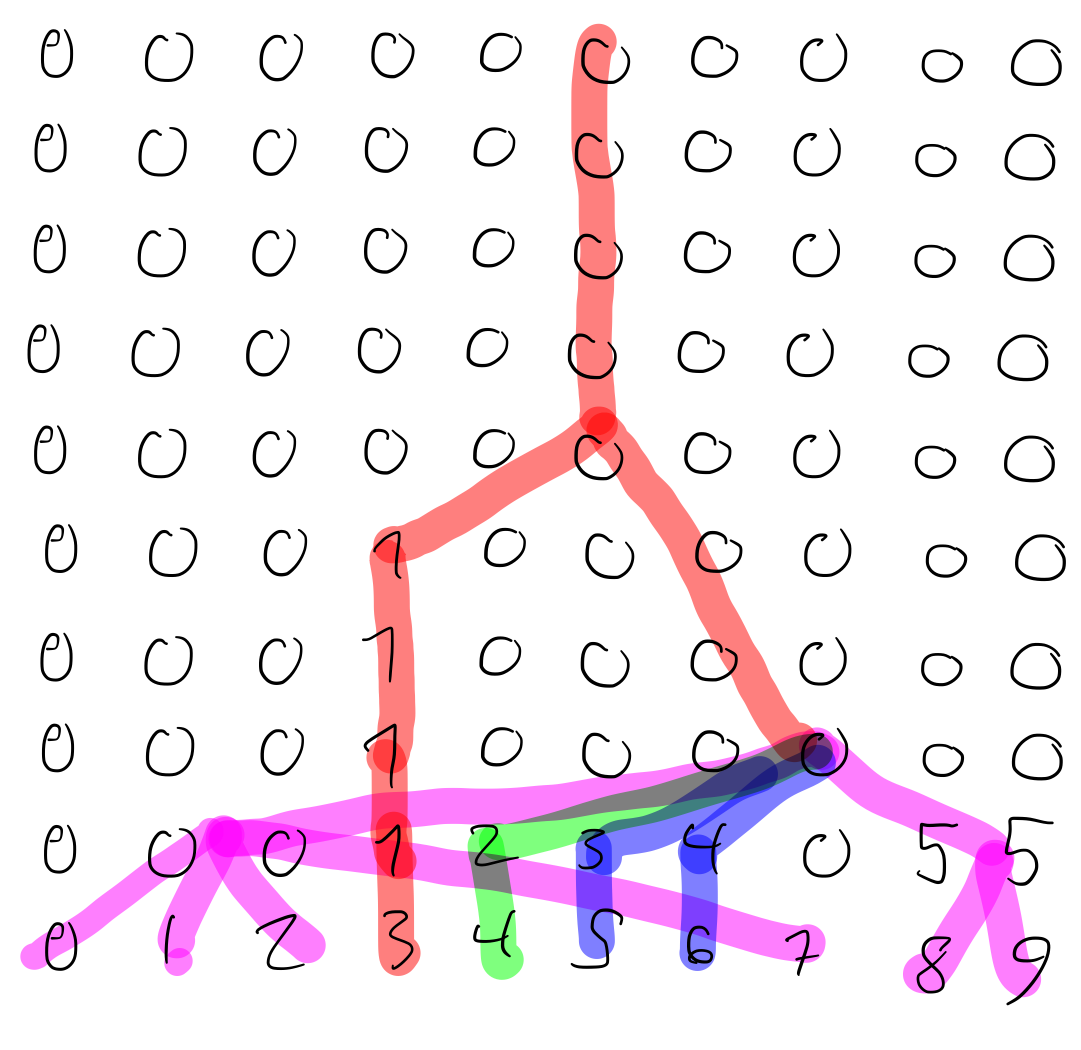
\includegraphics[width=.5\textwidth]{tree}
	\caption{How the tree structure is formed for the connected componenet vectors}
\end{figure}
For example, say $N=8$ and we have
\begin{align*}
	c(A^{(j)})=\{0, 0, 0 ,0, 1 ,1 ,1, 1\}\\
	c(A^{(j+1)})=\{0, 0, 0 ,0, 1 ,1 ,2, 2\}
\end{align*}
This means that $A^{(j)}$ has two connected components, ordered 0 (with vertices 1,2,3,4) and 1 (with vertices 5,6,7,8) and that $A^{(j+1)}$ has three connected components, ordered 0 (with vertices 1,2,3,4), 1 (with vertices 5 and 6) and 2 (with vertices 7 and 8).  Thus there is a branch from the connect component 1 in $A^{(j)}$ to the connected componenets 1 and 2 in $A^{(j+1)}$. By greedily repeating this iterative algorithm starting with $A^{(1)}$ \footnote{which has by definition only a single connected component and so $c(A^{(1)})=\{0, \cdots, 0\}$} as the root, we produce the tree of topics. Observe that at this stage, all the leaf nodes correspond to actual topics $t_n$. We formulate the topic vectors for the parent nodes by additive percolating up the tree. That is, for a given parent topic $\tau$ with children $\tau_1, \cdots, \tau_k$ we simply have 
$$\tau =\sum_i \tau_i $$
\begin{figure}
	\centering
	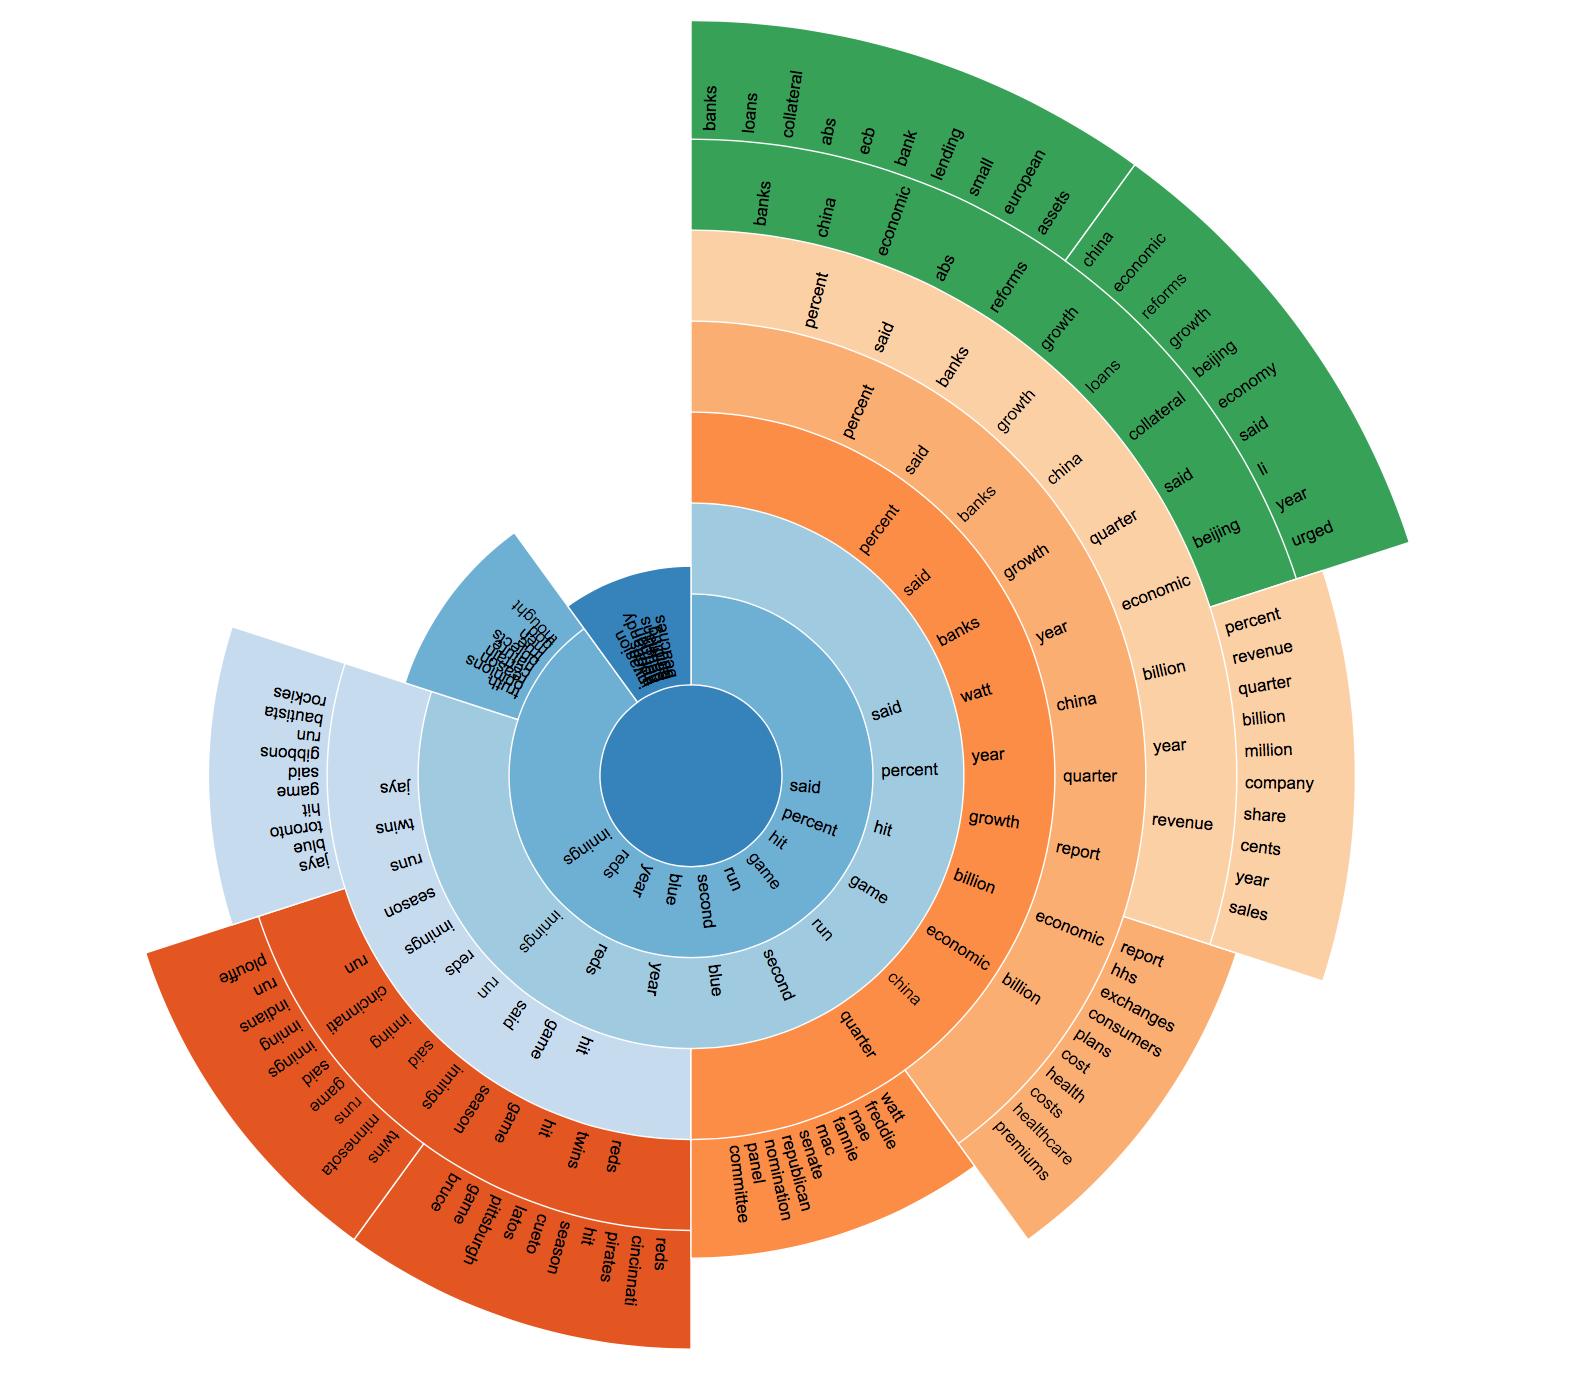
\includegraphics[width=.99\textwidth]{img}
	\caption{Screen shot of hierarhical topic model application for sample data set}
\end{figure}


\bibliographystyle{plain}

\bibliography{myBib.bib}


\end{document}